% TO-DO:  Kolmogorov complexity

\documentclass[15pt]{beamer}
\usepackage[CJKspace]{xeCJK}
%\usepackage{newtxtext,newtxmath}	% use Times Roman font
%\usefonttheme{serif}
\usefonttheme{professionalfonts}
%\setbeamertemplate{theorems}[numbered]
\setbeamertemplate{caption}{\insertcaption} 	% no `Figure' prefix before caption

\mode<presentation> {

%\usetheme{default}
%\usetheme{AnnArbor}
%\usetheme{Antibes}
%\usetheme{Bergen}
%\usetheme{Berkeley}
%\usetheme{Berlin}
%\usetheme{Boadilla}
%\usetheme{CambridgeUS}
%\usetheme{Copenhagen}
%\usetheme{Darmstadt}
%\usetheme{Dresden}
%\usetheme{Frankfurt}
%\usetheme{Goettingen}
%\usetheme{Hannover}
%\usetheme{Ilmenau}
%\usetheme{JuanLesPins}
%\usetheme{Luebeck}
\usetheme{Madrid}
%\usetheme{Malmoe}
%\usetheme{Marburg}
%\usetheme{Montpellier}
%\usetheme{PaloAlto}
%\usetheme{Pittsburgh}
%\usetheme{Rochester}
%\usetheme{Singapore}
%\usetheme{Szeged}
%\usetheme{Warsaw}

%\usecolortheme{albatross}
%\usecolortheme{beaver}
%\usecolortheme{beetle}
%\usecolortheme{crane}
%\usecolortheme{dolphin}
%\usecolortheme{dove}
%\usecolortheme{fly}
%\usecolortheme{lily}
%\usecolortheme{orchid}
%\usecolortheme{rose}
%\usecolortheme{seagull}
%\usecolortheme{seahorse}
%\usecolortheme{whale}
%\usecolortheme{wolverine}

%\setbeamertemplate{footline} % To remove the footer line in all slides uncomment this line
%\setbeamertemplate{footline}[page number] % To replace the footer line in all slides with a simple slide count uncomment this line
\setbeamertemplate{navigation symbols}{} % To remove the navigation symbols from the bottom of all slides uncomment this line
}

\usepackage{graphicx} % Allows including images
\usepackage{verbatim} % comments
% \usepackage{tikz-cd}  % commutative diagrams
% \newcommand{\tikzmark}[1]{\tikz[overlay,remember picture] \node (#1) {};}
% \usepackage{booktabs} % Allows the use of \toprule, \midrule and \bottomrule in tables
% \usepackage{amssymb}  % \leftrightharpoons
\usepackage{wasysym} % frownie face
\usepackage{newtxtext,newtxmath}	% Times New Roman font

\newcommand{\vect}[1]{\boldsymbol{#1}}
\newcommand*\sigmoid{\vcenter{\hbox{
\includegraphics{sigmoid.png}}}}

\makeatletter
\renewcommand{\boxed}[1]{\fbox{\m@th$\displaystyle\scalebox{0.9}{#1}$} \,}
\makeatother

%---------------------------- make slide margin narrower --------------------------------
\newcommand\Wider[2][3em]{%
	\makebox[\linewidth][c]{%
		\begin{minipage}{\dimexpr\textwidth+#1\relax}
			\raggedright#2
		\end{minipage}%
}%
}

%----------------------------------------------------------------------------------------
%	TITLE PAGE
%----------------------------------------------------------------------------------------

\title[AGI architectures]{论 AGI 的架构} % The short title appears at the bottom of every slide, the full title is only on the title page

\author{YKY 甄景贤} % Your name
\institute[] % Your institution as it will appear on the bottom of every slide, may be shorthand to save space
{
Independent researcher, Hong Kong \\ % Your institution for the title page
\medskip
\textit{generic.intelligence@gmail.com} % Your email address
}
\date{\today} % Date, can be changed to a custom date

\begin{document}

\frame{\titlepage}

%\begin{frame}
%\frametitle{Talk summary}
%\tableofcontents
%\end{frame}

%---------------- this is for when you're using \part's ----------------------------------
%\begin{frame}
%\frametitle{Summary}
%
%{\usebeamerfont*{frametitle} Part I %\usebeamercolor[fg]{frametitle}
% ~ ~ ~ Deep reinforcement learning}
%%\tableofcontents[part=1]
%
%\vspace{1.5cm}
%{\usebeamerfont*{frametitle} Part II %\usebeamercolor[fg]{frametitle}
% ~ ~ ~ Logical structure}
%%\tableofcontents[part=2]
%\end{frame}

%----------------------------------------------------------------------------------------
%	PRESENTATION SLIDES
%----------------------------------------------------------------------------------------

%------------------------------------------------

%\part{title}

%\section[Section]{}
%\frame{\sectionpage}

\begin{frame}
\frametitle{最简单的 AGI 架构}
\begin{itemize}
	\item 最简单的 AGI 架构是这样的:(它包含一个 recurrent 回路)
\begin{equation}
\vcenter{\hbox{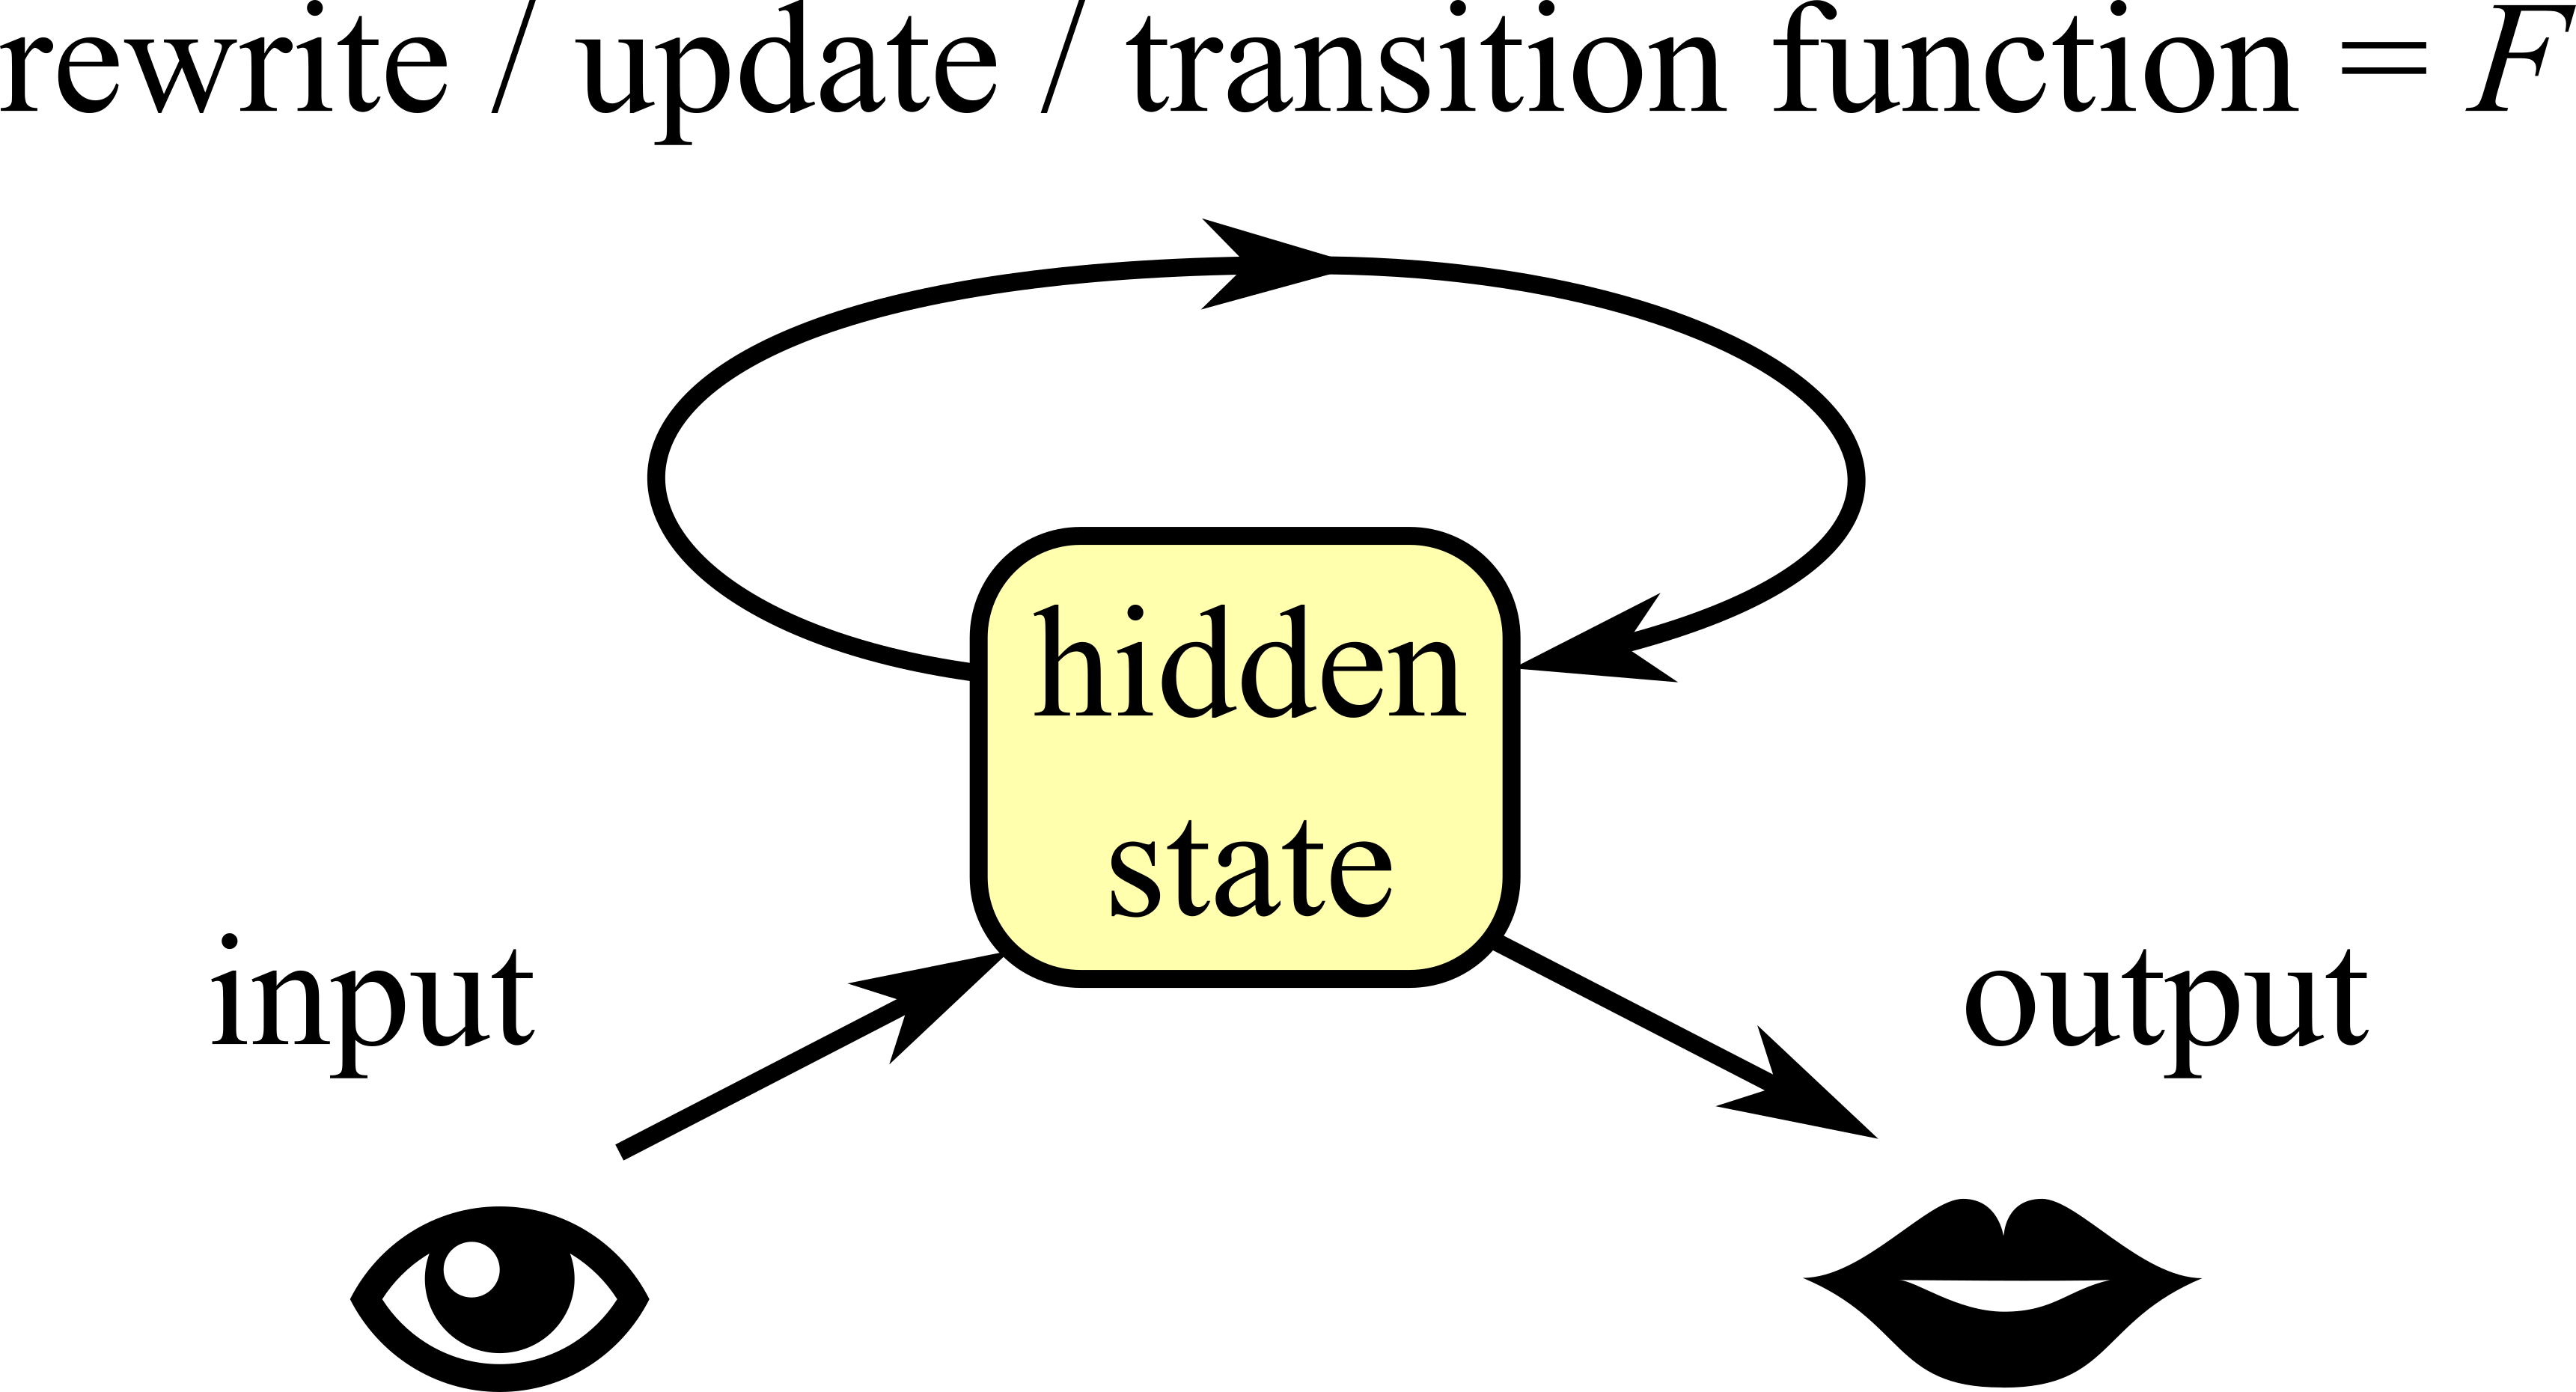
\includegraphics[scale=0.5]{minimal-architecture.png}}}
\end{equation}
	\item 它在 \textbf{强化学习} 的框架下,根据 Bellman 最优化条件,将 奖励 最大化
	\item Transition function $F$ 可以用一个 神经网络 实现
	\item 根据我先前解释过的 no free lunch 理论,这个架构的问题是缺乏 inductive bias,学习太慢
\end{itemize}
\end{frame}

\begin{frame}
\frametitle{No free lunch (NFL) 的迷思}
\begin{itemize}
	\item 根据 no free lunch 哲学,没有所谓「好」与「坏」的归纳偏好
	\item 只要能加速学习的,但又不 切掉 AGI,都是好 bias
	\item 但我又说,要用 逻辑结构 作为 bias; 这有没有矛盾?
	\item 例如,可以将 $F$ 的神经网络 变稀疏 (sparse),但保持 深度 (deep)
	\item 
\end{itemize}
\end{frame}


\begin{frame}
\frametitle{Topos}
Topos 是指一个能够在里面「做逻辑」的范畴。 它起源於将 \textbf{集合论} 改写成 \textbf{范畴论} 的尝试。

\end{frame}

\begin{frame}
\frametitle{Representation theory}
\end{frame}

\begin{frame}
\frametitle{The end}
	\begin{center}
		多谢收看 \smiley{}
	\end{center}
\end{frame}

\begin{comment}

\begin{frame}
\frametitle{References}
\footnotesize{
\begin{thebibliography}{99} % Beamer does not support BibTeX so references must be inserted manually as below
\bibitem[]{} Bart Jacobs (1999)
\newblock Categorical logic and type theory
% \newblock \emph{North Holland, Studies in logic} v141.

\bibitem[]{} Robert Goldblatt (2006)
\newblock Topoi -- the categorical analysis of logic

\end{thebibliography}
}
\end{frame}

\end{comment}

\end{document} 